\chapter{Results}

\begin{table}[H]
    \centering
    \begin{tabularx}{\textwidth}{X X}
        \toprule
        Metric & Value \\
        \midrule
        Number of Samples & 24,946\\
        Successfully Predicted & 100\%\\
        Mean Absolute Error (MAE) & 0.29 \\
        Root Mean Squared Error (RMSE) & 0.39 \\
        Median Absolute Error & 0.23 \\
        Maximum Absolute Error & 4.94 \\
        $R^2$ & 0.92 \\
        Pearson $r$ & 0.96 \\
        Mean Inference Time & 53.13 ms \\
        Mean Round Trip Time & 237.97 ms \\
        \bottomrule
    \end{tabularx}
    \caption{Performance metrics on the test set.}
    \label{tab:performance_metrics}
\end{table}

\begin{figure}[H]
    \centering
    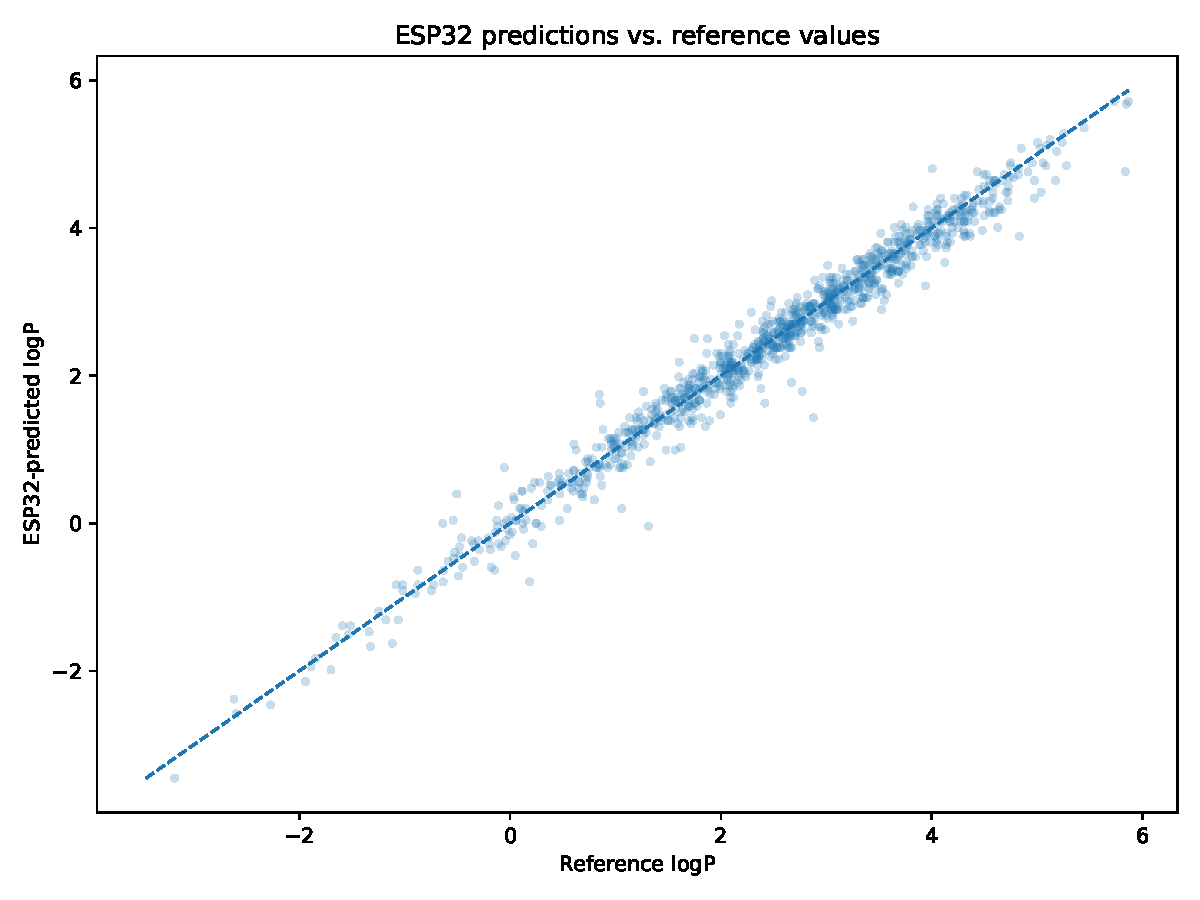
\includegraphics[width=0.8\textwidth]{Code/Results/figures/scatter_actual_vs_predicted.pdf}
    \caption{Scatter plot of true vs. predicted \gls{logp} values for the test set. The diagonal line represents perfect predictions. The "plateau" of predictions at the top right is due to a clamping effect caused by the quantization process.}
    \label{fig:scatter_plot}
\end{figure}

\begin{table}[H]
    \centering
    \begin{tabularx}{\textwidth}{X X}
        \toprule
        Metric & Value \\
        \midrule
        Within 0.25 logP units & 53.12\% \\
        Within 0.50 logP units & 83.10\% \\
        Within 1.00 logP units & 98.06\% \\
        \bottomrule
    \end{tabularx}
    \caption{Percentage of predictions within certain absolute error thresholds.}
    \label{tab:error_thresholds}
\end{table}

\begin{figure}[H]
    \centering
    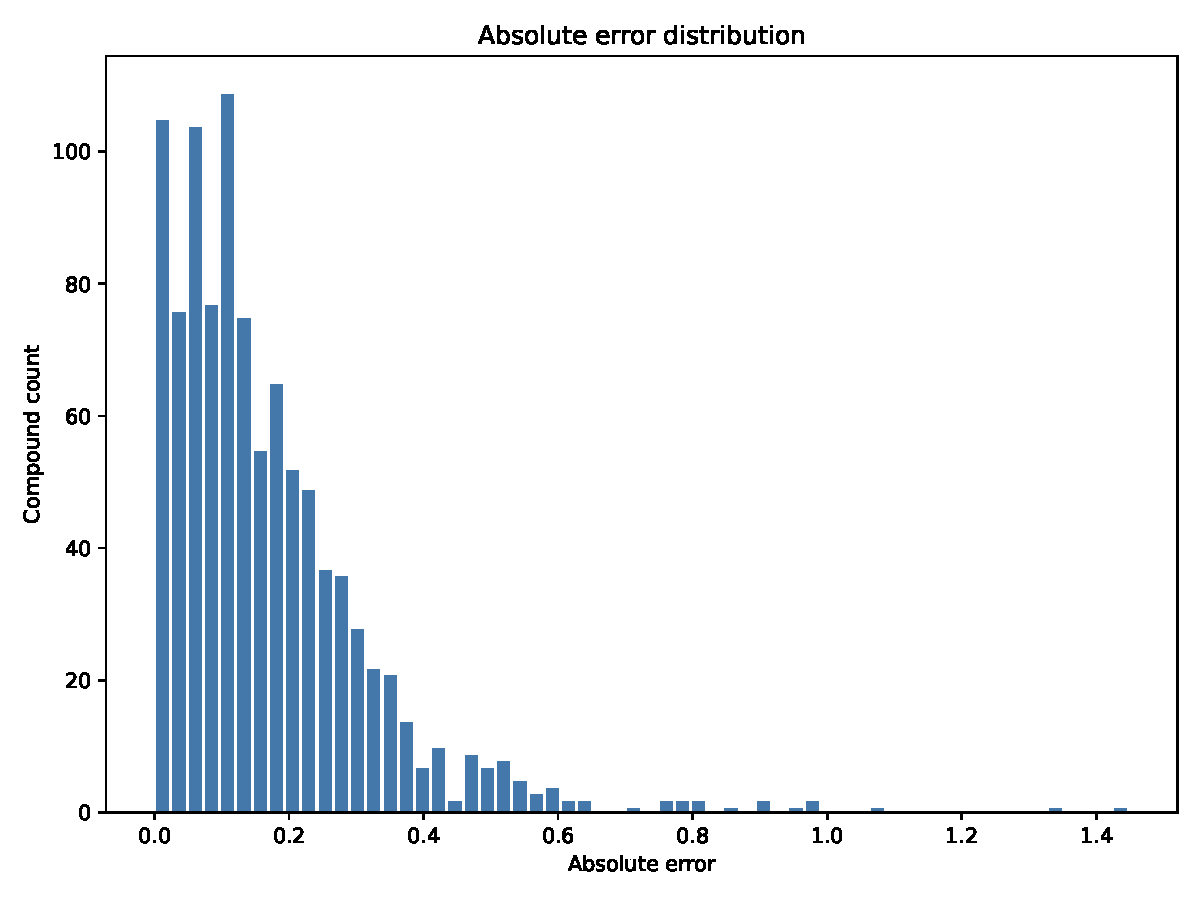
\includegraphics[width=0.8\textwidth]{Code/Results/figures/absolute_error_histogram.pdf}
    \caption{Histogram of absolute errors between predicted and true \gls{logp} values. The majority of predictions have an absolute error below 0.5, with a long tail extending to higher errors.}
    \label{fig:error_histogram}
\end{figure}

\begin{figure}[H]
    \centering
    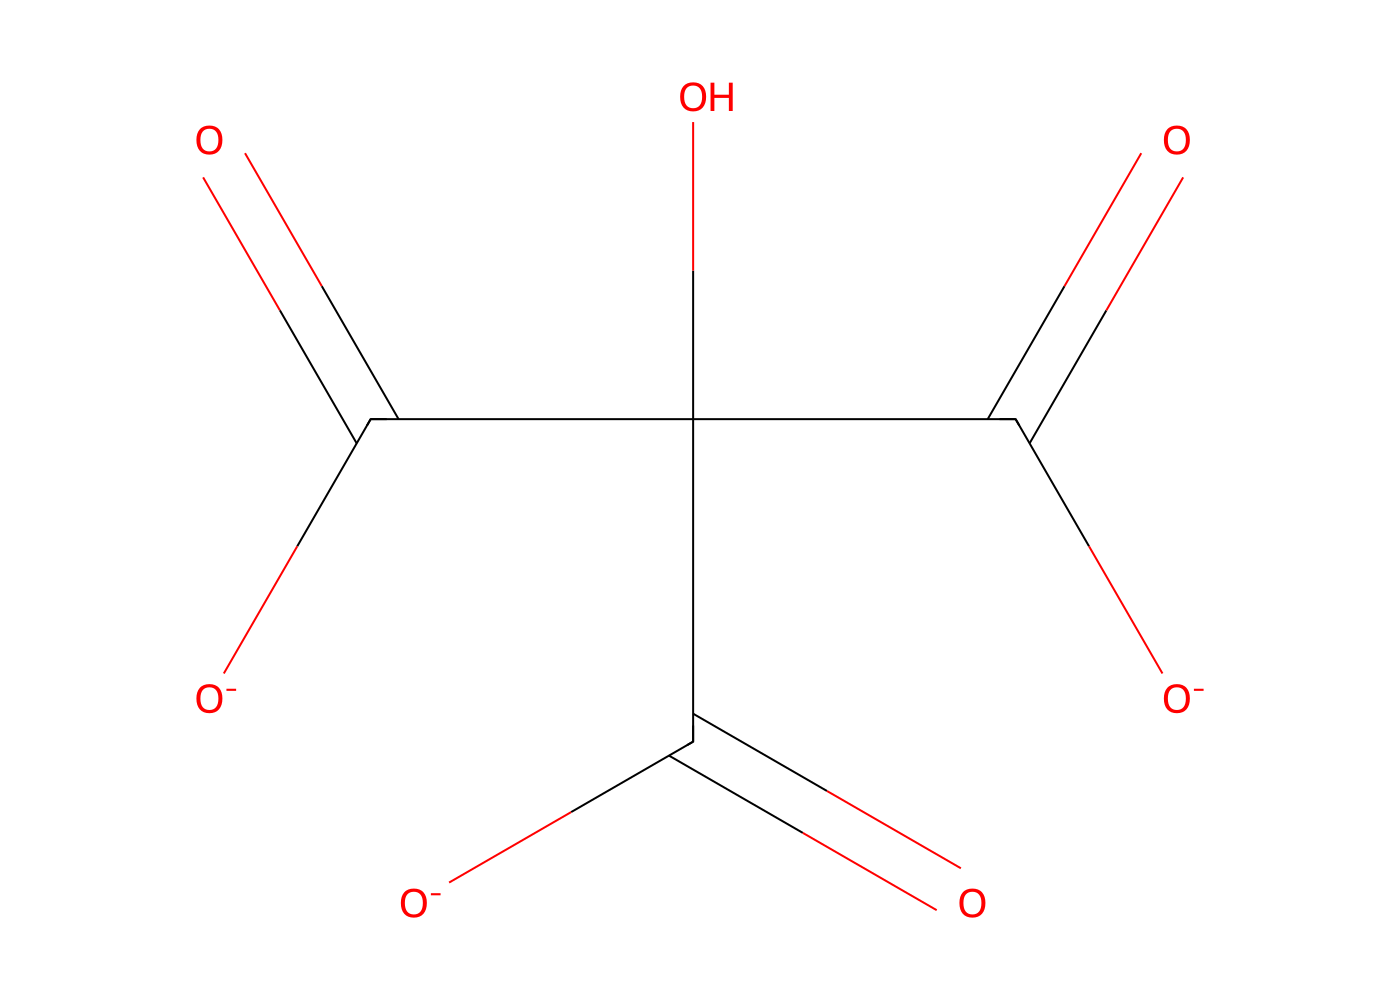
\includegraphics[width=0.5\textwidth]{Code/Results/molecules/worst_case.png}
    \caption{Citrate ion, the molecule with the worst prediction error (4.94). The ground truth logP is -6.03, while the predicted logP is -1.09.}
    \label{fig:worst_case_molecule}
\end{figure}